\section{Contextual Dynamics}
\label{sec:condy}



The structure of our stepper is shown in Figure \ref{fig:structure}. We use the similar structure developed by \citet{cong_implementing_nodate}. The expression is first decomposed into many independent evaluation contexts. Then, user may choose one of them to step. And the stepper will compose them into final result. For example, in Figure \ref{fig:multiple}, we have 3 evaluation contexts highlighted as green boxes. And when we click the second one, only the expression in second box is evaluated and composed into the whole expression.

\begin{figure}[htbp]
  \centering
  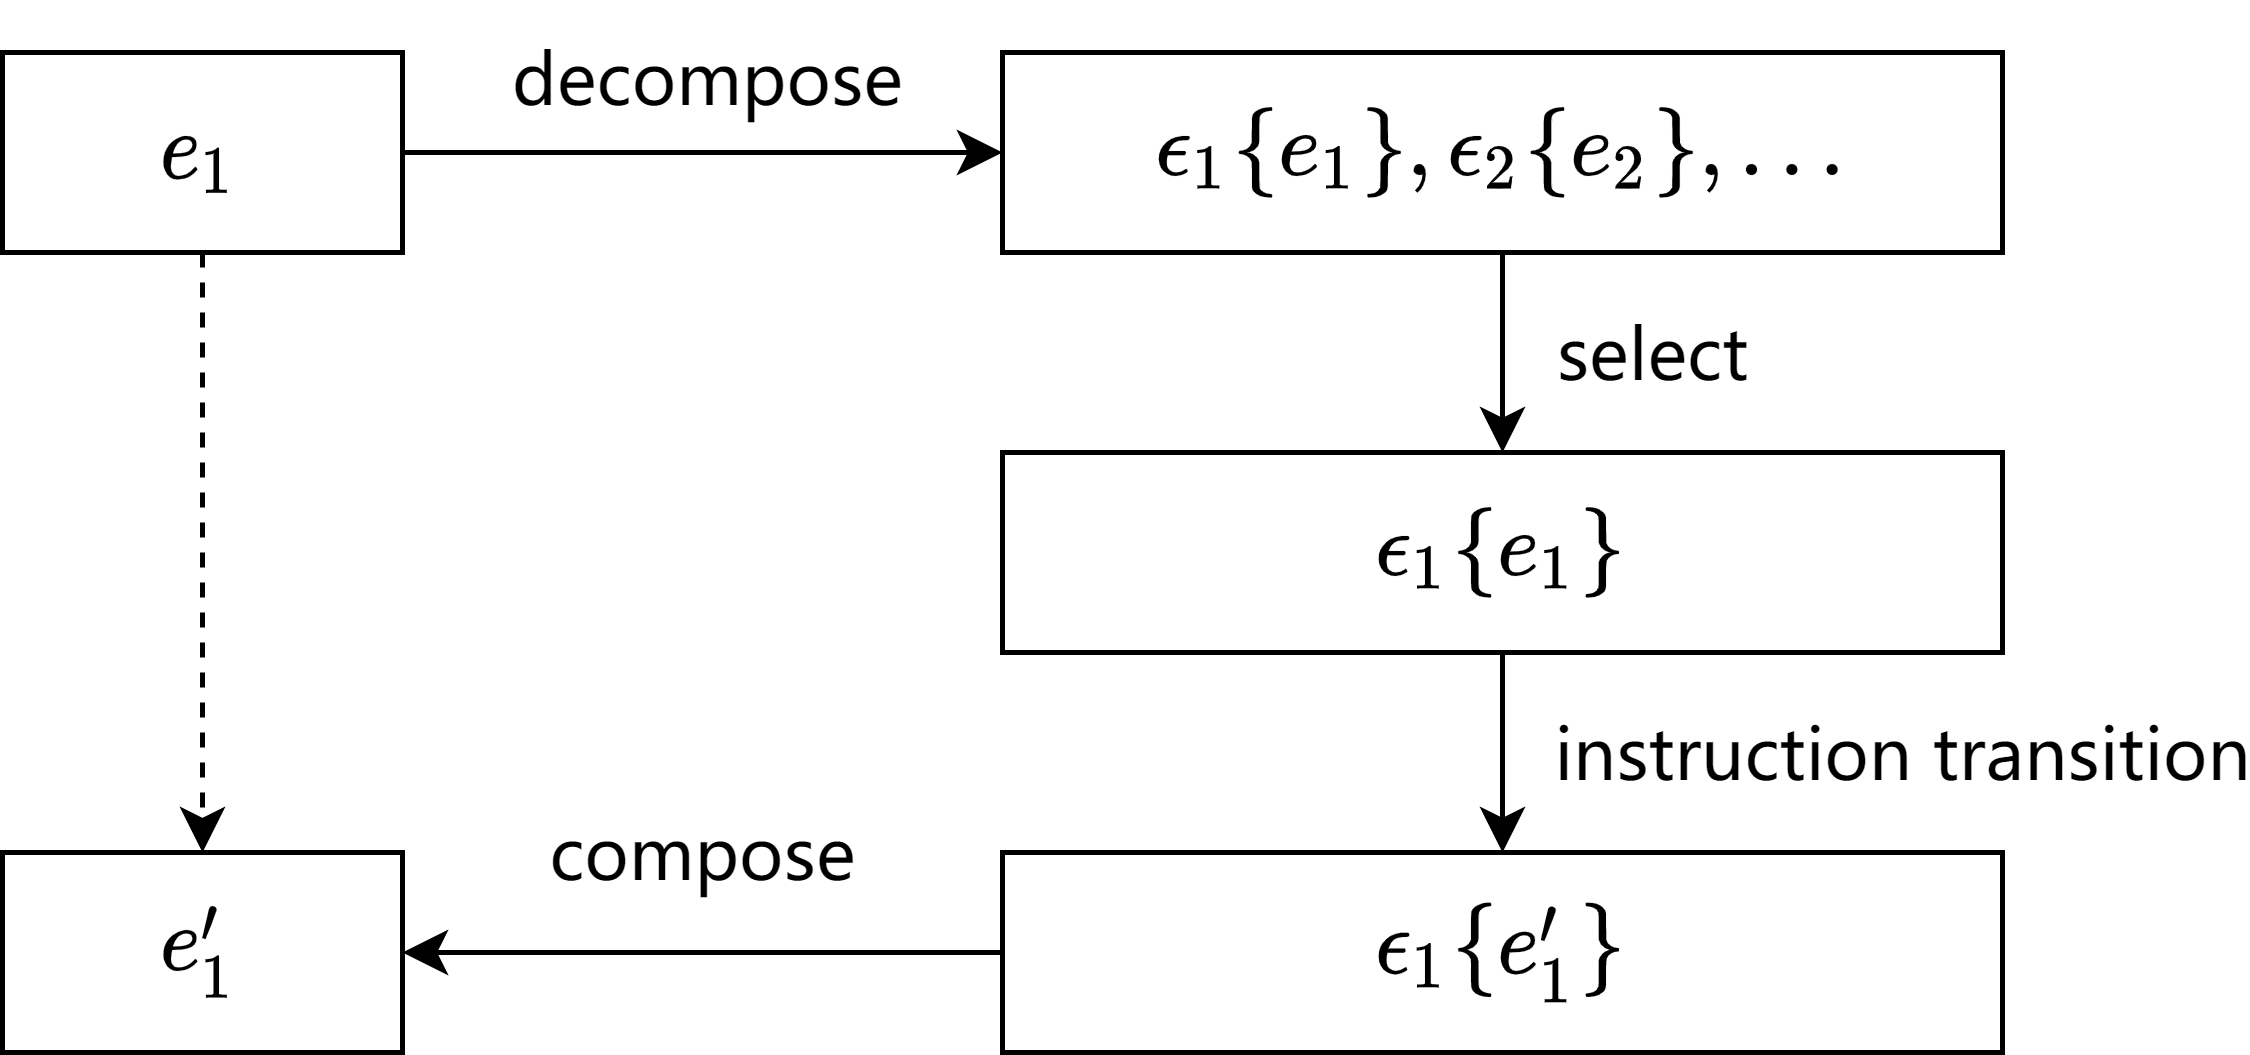
\includegraphics[width=0.5\textwidth]{img/struct.png}
  \caption{Structure of stepper}
  \label{fig:structure}
\end{figure}

We now formally define the instruction transition judgement. We use $\htrans{e_1}{e_2}$ as instruction transition judgement. Figure \ref{fig:decompose} shows some of the transition judgements.

% As what Section \ref{sec:pause} discussed, in \Hazel, we have four types of expressions: $\mathtt{boxedvalue}$, $\mathtt{indet}$, $\mathtt{final}$, and $\mathtt{paused}$. The instruction transition can be implemented to provide the type of the expressions. Therefore, we can easily know whether an expression is final, paused or steppable.

Then, we formally define the evaluation context. Unlike the regular evaluation context, the decompose function will return a list of contexts. The decompose function is defined recursively. Figure \ref{fig:decompose} provides some of inference rules for decompose function.

\begin{figure}[htbp]
  \vspace{-3px} 
  \fbox{ $\htrans{e}{e'} $}~~\text{$e$ takes an instruction transition to $e'$}\hfill
  \begin{subequations}
  \label{eqns:instr_trans}
    \begin{mathpar}
        %\hfill
        \inferrule[]{\isFinal{e_2}
            }{
              \htrans{\hap{\lamfunc{x}{e_1}}{e_2}}{[e_2/x]e_1}
            }
        %\hfill
    \end{mathpar}
  \end{subequations}

$\arraycolsep=4pt\begin{array}{lll}
\text{EvalCtx}~~ \epsilon & ::= &
  \circ  ~\vert~
  \hap{\epsilon}{e} ~\vert~
  \hap{e}{\epsilon} ~\vert~
  \hhole{\epsilon} ~\vert~
  \epsilon + e ~\vert~
  e + \epsilon
\end{array}$

\fbox{ $\hdecom{e}{[\hcontext{\epsilon_1}{e_1}, \hcontext{\epsilon_2}{e_2}, \cdots]} $}~~\text{$e$ is decomposed into contexts $\hcontext{\epsilon_1}{e_1}$, $\hcontext{\epsilon_2}{e_2}$, $\cdots$}\hfill
  \begin{subequations}\label{eqns:decompose}
  \begin{mathpar}
      \hfill
      \inferrule[DFinal]{\isFinal{e}
          }{
            \hdecom{e}{[]}
          }\hfill
      \inferrule[DApFinal]{\isFinal{e_1} ~~\isFinal{e_2}}{\hdecom{\hap{e_1}{e_2}}{[\hcontext{\circ}{\hap{e_1}{e_2}}]}}
      \hfill\hfill
  \end{mathpar}
  \begin{mathpar}
    \hfill
      \inferrule[DAp]{\hdecom{e_1}{[\hcontext{\epsilon_1}{e_1'}, \cdots]}\\ \hdecom{e_2}{[\hcontext{\epsilon_2}{e_2'}, \cdots]}}{\hdecom{\hap{e_1}{e_2}}{[\hcontext{\hap{\epsilon_1}{e_2}}{e_1'}, \cdots, \hcontext{\hap{e_1}{\epsilon_2}}{e_2'}, \cdots]}}
      \hfill\hfill
  \end{mathpar}
  \begin{mathpar}
    \hfill
    \inferrule[DHole]{\hdecom{e}{[\hcontext{\epsilon}{e'}, \cdots]}}{\hdecom{\hhole{e}}{[\hcontext{\hhole{\epsilon}}{e'}]}}
      \hfill
      \inferrule[DAdd]{\hdecom{e_1}{[\hcontext{\epsilon_1}{e_1'}, \cdots]}\\ \hdecom{e_2}{[\hcontext{\epsilon_2}{e_2'}, \cdots]}}{\hdecom{(e_1 + e_2)}{[\hcontext{(\epsilon_1 + e_2)}{e_1'}, \cdots, \hcontext{(e_1 + \epsilon_2)}{e_2'}, \cdots]}}\hfill\hfill
  \end{mathpar}
\end{subequations}
\hrule
\caption{Insturction transition and decomposition}
  \label{fig:decompose}
  \vspace{-5px}
\end{figure}


For example, we have an expression $e_0 = 4 + 1 + (5 + 6)$. First, we know that $\hdecom{4 + 1}{[\hcontext{\circ}{4 + 1}]}$ and $\hdecom{5 + 6}{[\hcontext{\circ}{5 + 6}]}$. So, According to $\mathtt{DAdd}$ rule, we have,
$$
\hdecom{4 + 1 + (5 + 6)}{[\hcontext{(\circ + (5 + 6))}{4 + 1}, \hcontext{(4 + 1 + \circ)}{5 + 6}]}.
$$
User may choose second one so that the stepper will first evaluate $5 + 6$ and put result into mark. Hence, we get $4 + 1+ 11$ finally.